\chapter{Conclusions and Future Work}
\section{Conclusions}
Bas-relief is an art form part way between 3D sculpture and 2D painting. We present a new approach for generating a bas-relief from a single Chinese brush painting automatically. \\
Based on layer decomposition , our approach can effectively extract brush strokes from 2D paintings and generate the individual depth maps for bas-relief. We show the superiority of our results by comparing it with alternative works in each step.\\ \\
In summary,our contributions include:
\newline
(1) Extraction of brush strokes. We develop a novel method to extract brush strokes based on paint colors analysis and layer decomposition.  Comparing with previous method brush stroke extraction methods, our method is capable of extracting overlapped brush strokes automatically without the prior knowledge of brush strokes and has higher accuracy. 
\newline
(2) Bas-relief generation of each brush stroke. We develop a novel method which may entirely generated every stroke to a correspond bas-relief surface(a depth map). By doing so, we preserve the feature of the input painting well.\\
(3) Bas-relief generation from opacity. In contrast with previous 2D image based methods, our method use opacity instead of intensity to generate bas-relief, which can better preserve the feature of input painting.\\ 
(4)Our brush stroke extraction technique has other potential uses. We demonstrate the utility of the decomposed brush strokes for image editing. See section \ref{editing}.\\
Our experiments show that our method is able to produce convincing bas-reliefs from a variety of Chinese brush paintings (with human, animal, flower,etc.)  and even some other suitable styles including rosemaling paintings. \\   
\section{Future Work}

Although the proposed algorithm is already capable to generate a bas-relief from a single Chinese brush painting automatically, there is still further work to do, including refinement of our method based on the limitations,and use it in other applications.

\subsection{Refine Current Algorithm}
One future work is to further improve the performance of current algorithm. As we mentioned in section \ref{result}, there are two main limitation: (1) With wrongly picked paint colors, the layer decomposition may not preserve or separate the brush strokes. (2) When brush strokes highly blended with  multiple painting colors, it fails to be extracted faithfully by our current method. \\
We plan to investigate methods to automate the estimation of better color selection from the image contents, e.g., by analyzing the local features. Second, we would study how color composition equation would influence our brush stroke extraction, and refine our method based on it.  

\subsection{Application  }
\textbf{3D painting system}\newline
The concept of 3D painting system was introduced for more than two decades ago.  Hanrahan \cite{hanrahan1990direct} firstly present a 3D painting system that capable of painting on 3D models, but their work didn’t put transparency and fine detailed painting in consideration. \\
From works of  Daily et al. \cite{daily19953d}, 3D painting applied texture map for painting details effect. However, distortion or seams would happen due to 2D parametrization. Meier [1996] first proposed generating brush strokes attached to 3D objects.  Deep Canvas \cite{katanics2003deep}, firstly projected painted strokes on the object’s surface and dynamic 3D camera can be applied which is hard to achieve using traditional 2D paintings. The WYSIWYG NPR system \cite{kalnins2002wysiwyg} focused on algorithmic rendering techniques, which enable artist to achieve silhouette stylization and control hatching directly via a painting interface. Maya Paint Effects (Paint Effects 2011) also projects painted strokes onto the surface of scene geometry and uses them as seed points to create new geometric primitives such as grass or flowers.

\begin{figure}[H]
	\centering
	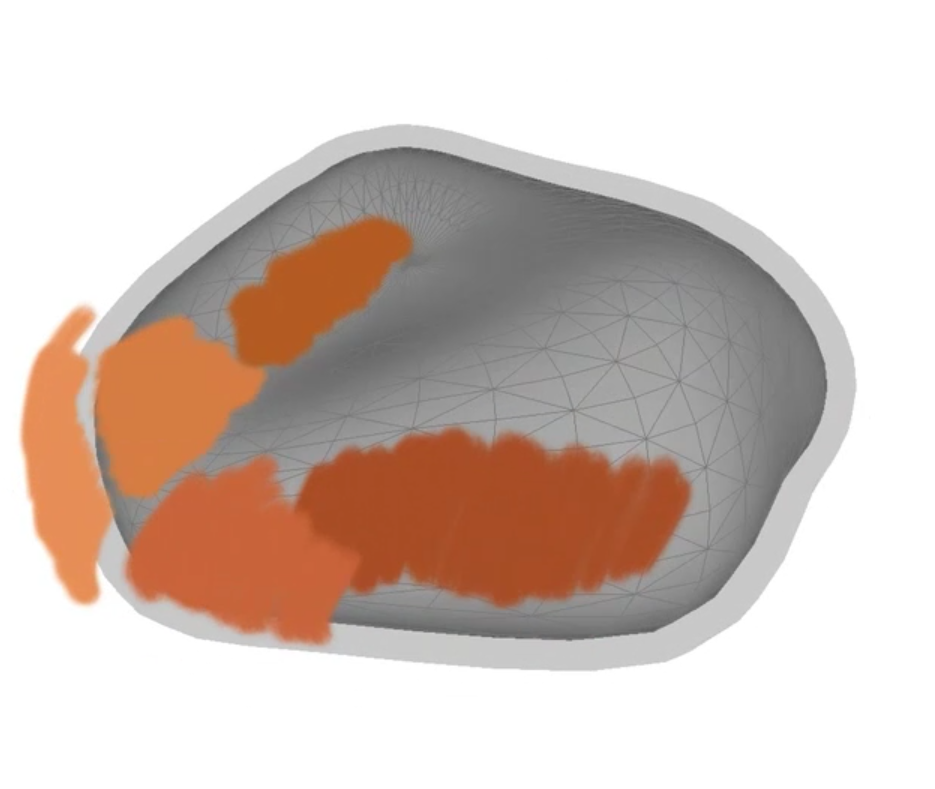
\includegraphics[width=10cm]{level_set.png}
	\caption{3D brush painting on surface level set}
	\label{level set}
\end{figure}

More recently, Overcoat \cite{schmid2011overcoat} introduced an implicit canvas for 3D painting, which enable creating approximate 3D proxy geometry to shape the implicit canvas, it allows us to implement tools for painting along level set surfaces or across different level sets. which means we can project parametric strokes onto the underlying 3D models as showed in Figure \ref{level set}.
These painting systems are focusing on how to paint on surface of known models. In CanvoX \cite{kim2017canvox} extended painting surface to volumetric painting, with GPU-based Octree \cite{lefebvre2005octree}.

With the rapid development of VR systems, it is natural to enable artists to paint in 3D space. In CavePainting \cite{keefe2001cavepainting} firstly create 3D analogy of 2D brush strokes, to create 3D works in a Cave environment. Softwares like Tilt Brush (1) and Quill (2) have recently surged and are now widely accepted by artists to be positioned as a new art form kim's work \cite{kim2017canvox}. For these painting system, quad strips are rendered as painting strokes, which are fully based on user input. \\
\textbf{Application in 3D Painting}\\
With the increasing popularity and development of virtual reality, digital painting on 2D canvases is now being extended to 3D spaces. 3D painting as a new art form are now widely accepted among artists. Software on VR platform make 3D painting more and more intuitive for 2D painters.   
We aim to build a system which enable artist to transfer a given 2D Chinese painting to 3D painting, in a way that gives creative freedom to the artist while maintaining an acceptable level of controllability based on the given 2D Chinese painting.\\
We address this problem into four main steps: \\
First, segment strokes from the given 2D Chinese painting. Since in 3D painting, strokes are placed in 3D space based on user input, to mimic such effect, successful strokes segmentation is quite essential. Brush strokes may have high diversity of colour, so layer decomposition may need to be applied. \\
Second, stroke refinement, since brush strokes may be over segmented or under segmented, stroke need to be refined. A refinement method based on user input need to be applied. \\
Third, transfer 2D strokes to 3D strokes, simulate the effect the 3D stroke with supplied 2D stroke, and 3D volumetric painting would be applied \cite{kim2017canvox}. \\
Fourth, 3D strokes placement, based on the layer order and user inputs, we place and blend 3D strokes in 3D space. \\
\section{Proposed timescale for the work:}
Refine the first step of layer decomposition, with the coherent edge of the given 2D brush painting, iteratively calculate the paint colors. (6 weeks)\\
Stroke segmentation into a hierarchical structure, currently,  hierarchical clustering are in consideration. (4 weeks)\\
Design the user interface for refine the stroke segmentation. (4 weeks)\\
With given segmented strokes, generate corresponding mesh, with detail and style preserved. (4 weeks)\\
Design the interface for user input, in which high relief can be placed naturally in 3D space while maintaining an acceptable level of controllability. (4 weeks)\\
Optimization.  (4 weeks)
\newline

\begin{table}[H]
	\centering
	\caption{ Schedule of Future Research Plan}
	\label{my-label}
	\begin{tabular}{|l|l|}
		\hline
		\textbf{Research Activity} & \textbf{Target Completion Date} \\ \hline
		\begin{tabular}[c]{@{}l@{}}Refine current algorithm \end{tabular} & 11/12/2017 \\ \hline
		\begin{tabular}[c]{@{}l@{}}Design the user interface for refine the\\ stroke segmentation.\end{tabular} & 01/3/2018 \\ \hline
		\begin{tabular}[c]{@{}l@{}}3D stroke analogy design and 3D stroke\\ placement design .\end{tabular} & 01/04/2018 \\ \hline
		Optimization. & 01/05/2018 \\ \hline
		Write final Thesis for PhD graduation & 01/10/2018 \\ \hline
	\end{tabular}
\end{table}